\chapter{Question2}
\section{问题概述}
%
%%对问题的直观描述
%
本问题要求实现Minimax算法,其中正方只有一个智能体,即吃豆人,但是反方,即幽灵,可能有多个。
%
%对项目已有代码的阅读和理解
%
%
%解决问题的思路和想法
%
\section{算法设计}
%
%用自己的语言描述解决问题所使用的算法的原理及功能,设计思路和算法流程图
%
由于可能有多个反方,所以在博弈树中,对应着正方的每一层下方都紧接着$n$层反方的结点,其中$n$为反方的个数。同时,
题目明确要求当层数到达给定值后,便使用评估函数,其中,“一层”对应着一轮游戏,即吃豆人和所有的幽灵都轮流各走了一步。

\begin{algorithm}[h]
    \SetKw{maximize}{maximize} 
    dummy,action = \maximize(gameState,1)\tcp*[h]{这里无需返回的分数}\;
    \Return{action}
    \caption{Minimax(gameState)}
\end{algorithm}

\begin{procedure}[h]
    \KwOut{bestScore,bestAction}
    \SetKw{in}{in}
    \SetKw{minimize}{minimize}
    \tcp*[h]{给定状态和对应深度,返回从当前状态出发所能达到的最佳分数和对应的动作}\;
    actions = gameState.getLegalActions()\;
    ghostNum = gameState.getNumAgent - 1\;
    \If{depth > depthLimit or actions == None}
    {\Return{evaluationFunction(gameState),None}\tcp*[h]{无法继续行动,直接返回当前状态的分数}}
    bestScore = $-\infty$\;
    bestAction = None\;
    \ForEach{action \in actions}
    {
        next = gameState.generateSuccessor(gameState,action)\tcp*[h]{获取下一个状态}\;
        score,dummy = \minimize(next,1,ghostNum,depth)\tcp*[h]{这里并不需要返回的动作}\;
        \If{score > bestScore}
        {
            bestAction = action\;
            bestScore = score\;
        }
    }
    \Return{bestScore,bestAction}
    \caption{maximize(gameState,depth)}
\end{procedure}

\begin{procedure}[h]
    \KwOut{bestScore,bestAction}
    \SetKw{in}{in}
    \SetKw{minimize}{minimize}
    \tcp*[h]{给定状态和对应深度,返回从当前状态出发所能达到的最佳分数和对应的动作}\;
    actions = gameState.getLegalActions()\;
    \If{depth > depthLimit or actions == None}
    {\Return{evaluationFunction(gameState),None}\tcp*[h]{无法继续行动,直接返回当前状态的分数}}
    bestScore = $\infty$\;
    bestAction = None\;
    \ForEach{action \in actions}
    {
        next = gameState.generateSuccessor(gameState,action)\tcp*[h]{获取下一个状态}\;
        \eIf{ghostNo == ghostNum}
        {
            score,dummy = \maximize(next,depth+1)\tcp*[h]{当前智能体是最后一个幽灵,下一层为吃豆人}
        }
        {
        score,dummy = \minimize(next,ghostNo+1,ghostNum,depth)\tcp*[h]{这里并不需要返回的动作}
        }
        \If(\tcp*[h]{对于幽灵而言,目标是让吃豆人的分数尽可能的低}){score < bestScore}
        {
            bestAction = action\;
            bestScore = score\;
        }
    }
    \Return{bestScore,bestAction}
    \caption{minimize(gameState,ghostNo,ghostNum,depth)}
\end{procedure}

Minimax算法的核心是递归,并且使用的前提是博弈双方是理性的。maximize,minimize函数分别用于给出正反方的下一步以及对应的最优解的分数。
当无法继续行动时,当前状态是唯一可行的状态,自然是最优解。如果可以正方行动,那么在行动前,由于反方是理性的,正方需要枚举所有可能的行为,通过调用minimize
推算反方的反应和最终的结果,并最终选取出最佳的下一步。反方亦然。特别之处在于有多位反方,由于算法中的score统一是指正方的分数,所以无论是调用minimize的反方,
还是最后一位调用maximize的反方,其选取下一步的依据都是让score最小。

如果不在指定的深度调用评估函数,那么Minimax算法可能会产生无穷深的博弈树,这是不可接受的。
\section{算法实现}
\begin{lstlisting}[emph={[3]currentGameState,gameState,depth},emphstyle={[3]\color{vscode_parametercolor}},emph={[4]GameState,MinimaxAgent},emphstyle={[4]\color{vscode_classcolor}}]
class MinimaxAgent(MultiAgentSearchAgent):
    def maximize(self, gameState: GameState, depth: int):
        actions = gameState.getLegalActions(0)
        if depth > self.depth or not actions:
            return self.evaluationFunction(gameState), None
        bestScore = -float('inf')
        bestAction = None
        for action in actions:
            next = gameState.generateSuccessor(0, action)
            score, _ = self.minimize(next, 1, gameState.getNumAgents() - 1, depth)
            if score > bestScore:
                bestAction = action
                bestScore = score
        return bestScore, bestAction

    def minimize(self, gameState: GameState, ghostNo: int, ghostNum: int, depth: int):
        actions = gameState.getLegalActions(ghostNo)
        if not actions:
            return self.evaluationFunction(gameState), None
        bestScore = float('inf')
        bestAction = None
        for action in actions:
            next = gameState.generateSuccessor(ghostNo, action)
            if ghostNo == ghostNum:
                score, _ = self.maximize(next, depth + 1)
            else:
                score, _ = self.minimize(next, ghostNo + 1, ghostNum, depth)
            if score < bestScore:
                bestScore = score
                bestAction = action
        return bestScore, bestAction

    def getAction(self, gameState: GameState):
        return self.maximize(gameState, 1)[1]
\end{lstlisting}
\section{实验结果}
%
%对试验结果进行详细展示,对每个问题展示测试截图,对于测试用例进行描述说明,对于为通过测试的用例结合自己的算法进行分析,可以结合调试过程进行分析
%
我成功获得了本问题的所有分数,图\ref{q2}为实验结果。测试用例分为以下几类:
\begin{enumerate}
    \item eval-function-lose-states,eval-function-win-states:测试内容为一颗高度为2的博弈树,目的在于测试算法是否判断当前状态为胜负已定,并调用评估函数
    \item lecture-6-tree,small-tree,minmax:测试内容为Minimax的基本功能
    \item vary-depth:在minmax测试的基础上,对深度的限制进行调整,以测试算法是否正确处理该情况
    \item x-ghost-xlevel:测试了多位反方和多层深度限制的情况
    \item tied-root:测试了算法是否正确处理得分相同的情况
    \item check-depth-x-ghost:重点测试了算法是否正确处理深度限制
    \item pacman-game:在小型迷宫中使用Minimax算法进行实战
\end{enumerate}
\begin{figure}[H]
    \centering
    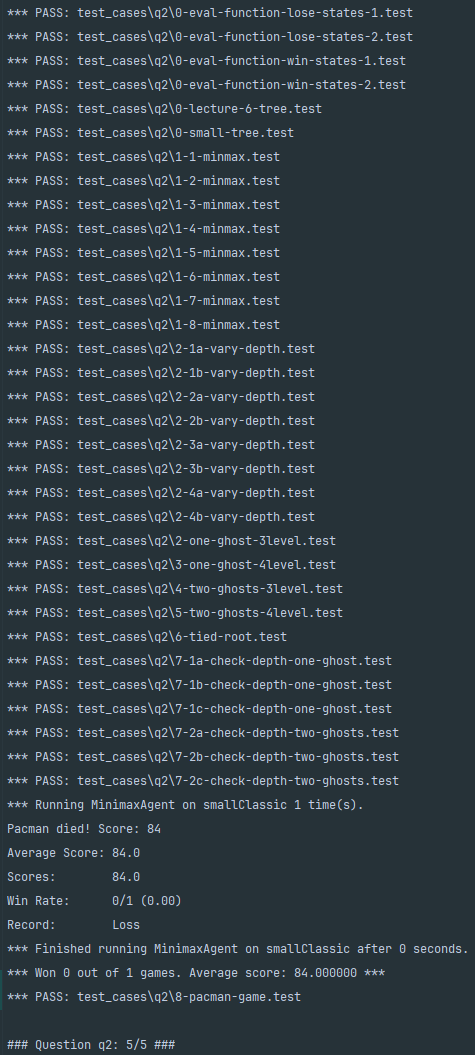
\includegraphics[scale = 0.8]{pic/q2.png}
    \caption{Question2实验结果}\label{q2}
\end{figure}
%
%在算法原理的基础上,结合代码,讲述算法的实现细节、和兴函数、模块输入输出,数据结构定义等内容
%
%
%对试验结果进行详细展示,对每个问题展示测试截图,对于测试用例进行描述说明,对于为通过测试的用例结合自己的算法进行分析,可以结合调试过程进行分析
%
%实验中遇到的问题及解决方案,收获和思考:对算法的理解、优缺点的评价、算法的适用场景
%
